\section{Design \& Implementation}\label{chapter.implementation}
\thispagestyle{plain}

\comment{[Backend/Off-Stage]}

This chapter aims to explain how \toolname \space is designed and implemented. \comment{It starts with a visualization and narrative of how data flows through the system.} It \comment{then} provides a description of how the system utilizes Selenium Grid. The implementation of the controller and some important details about this part of the system will then be presented. Further, the test allocation mechanism called \emph{Opti-X} will be explained with an accompanying example to illustrate how the mechanism works step-by-step will be presented. The chapter then explains how the database is structured in addition to the how it is accessed using Django libraries, before finally presenting some important implementation details about the dashboard.



%%%%%%%%%%%%%%%%%%%%%%%%%%%%%%%%
% SUBSECTION: Data Flow
%%%%%%%%%%%%%%%%%%%%%%%%%%%%%%%%
\comment{
\subsection{Data Flow}
\comment{Figure of how the data moves through the system.}
\improvement[inline]{TODO}
}

\subsection{Selenium Grid Integration}\label{section.selenium}

In \toolname, Selenium Grid works as the backbone of all interaction between the server and the remaining machines in the distributed system. It is used to establish connections and to perform test executions.

Setting up a Selenium Grid environment requires all involved machines to have a \emph{Selenium Standalone Server}, which is a file of the JAR (Java Archive) format, of the same version locally stored. The Selenium Standalone Server is started by executing a shell command.

A Selenium Grid Hub (server) can be started simply by executing the command in Listing \ref{listing.hub}, although it is possible to assign additional configuration, such as port and IP address, using flags. The default port number is 4444 for hubs and 5555 for nodes, so if nothing else is specified, these ports will be used. When the hub has started, the configuration can be viewed by opening \url{http://<hub-host>:4444/grid/console} in a browser.

\vspace{4mm}
\begin{lstlisting}[caption=Sample Shell Command for Starting Selenium Grid Hub, label={listing.hub}]
java -jar "C:/selenium-server-standalone-2.51.0.jar"
\end{lstlisting}

Starting Selenium Grid Nodes (test machines) require much longer and heavier commands, and thus more work. Also, the command must be customized, as it represents the configuration of the node and the distributed system. Therefore, a script devoted to gathering all necessary information and executing the command to start Selenium Standalone Server is included in this project. This script identifies which browsers are installed and what versions, as well as creating a unique identifier for each machines.

Selenium Grid currently does not offer a documented method of specifying which machine a test should be executed on. Instead, it maps the test to a node whose configuration that matches the desired specifications stated in the test, in regard to operating system, browser and sometimes even browser version. It was therefore necessary to find a way to work around this problem. This is done by utilizing a browser parameter called \emph{applicationName}, in which additional information can be added. A unique identifier based on the host ID, sequence number, and the current time, is created using Python's \emph{uuid} library. By adding as a requirement to a test that the applicationName should be equal to the uuid of a specific node, the test can be executed only on the machines with that uuid.

\vspace{4mm}
\begin{lstlisting}[caption=Sample Shell Command for Starting Selenium Grid Node, label={listing.node}]
java -jar "C:/selenium-server-standalone-2.51.0.jar" -role node -hubHost <hub-host> -uuid 1b234276-fc02-11e5-b752-080027f8a664 -browser "browserName=chrome, version=49.0.2623.110, applicationName=1b234276-fc02-11e5-b752-080027f8a664" -Dwebdriver.chrome.driver=path/to/chromedriver -browser "browserName=firefox, version=45.0, applicationName=1b234276-fc02-11e5-b752-080027f8a664"
\end{lstlisting}

Listing \ref{listing.node} shows an example of a command that will start a Selenium Grid Node with Chrome and Firefox installed, and with uuid \emph{1b234276-fc02-11e5-b752-080027f8a664}. Once the node is connected to the hub, the configuration can be retrieved as a JSON string from \url{http://<Hub Hostname/IP>:4444/grid/api/proxy?id=http://<Node IP>:5555}.

\comment{\info[inline]{Maybe start by explaining exactly Selenium Grid works and is used. How the hub and the nodes are started (cmd), how platform and version no and installed browsers and version nos are retrieved and included, how the distributed environment works. How a JSON object is retrieved from "10.0.0.6:4444/grid/api/proxy?id=http://10.0.0.10:8989" or whatever to check node settings/abilities. Explain briefly how Selenium WebDriver works.}}





%%%%%%%%%%%%%%%%%%%%%%%%%%%%%%%%
% SUBSECTION: Controller
%%%%%%%%%%%%%%%%%%%%%%%%%%%%%%%%
\subsection{Controller}

\begin{figure}[h]
    \centering
    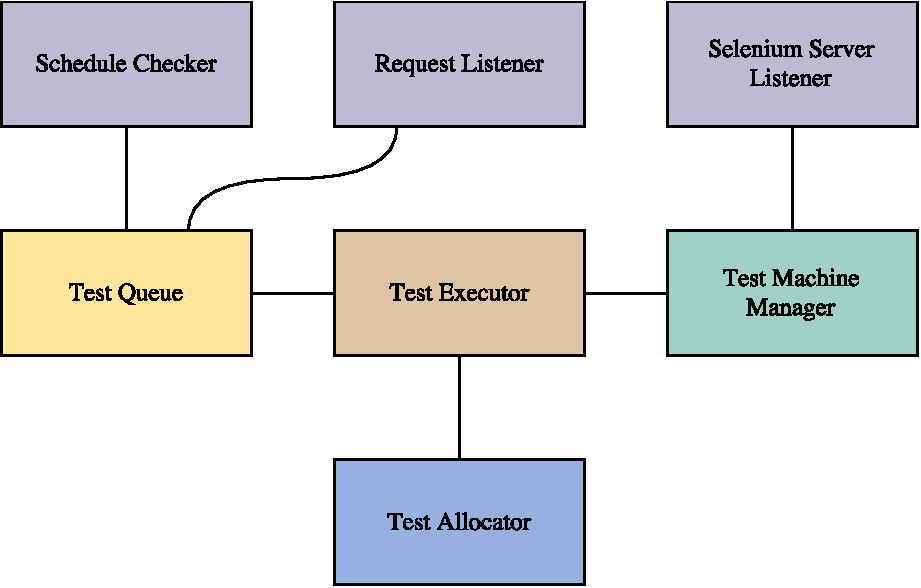
\includegraphics[width=\textwidth]{figures/new/controller3.pdf}
    \thisfloatpagestyle{plain}
    \caption{Controller Structure}
    \label{fig.controller_structure}
\end{figure}


\noindent The \emph{controller} consists of multiple processes running in different threads. Figure \ref{fig.controller_structure} shows the inner structure. Each of the modules in the figure will be explained in this Section.

\subsubsection{Selenium Server Listener}
After starting the Selenium Grid Hub as described in Section\ref{section.selenium} using configuration details found in the configuration file, the main job of the Selenium Server Listener is to listen to the output from the Selenium Standalone Server. This means that when a node connects or disconnects to the system, the Selenium Server Listener is notified. When one of these events happens, it sends notice to its instance of the Test Machine Manager.

\subsubsection{Test Machine Manager}

\improvement[inline]{TODO (Might re-implement this, so will wait with writing this subsection.)}

\subsubsection{Request Listener}

All test executions managed by \toolname \space are either requested for immediate execution or scheduled ahead of time. There are two different modules in the controller each handling one of these.

The \emph{Request Listener} constantly listens to a port specified in the configuration file. When a user triggers the \emph{Execute Now} action from the dashboard, all necessary information about the tests being requested for execution is packed as a \emph{JSON} string and sent to the controller using a TCP/IP protocol in Python's \emph{socket} library.

Upon receiving a request, the request listener unpacks the JSON string and creates a list of corresponding \emph{test} objects. The list is then forwarded to the \emph{queue}.


\subsubsection{Schedule Listener}
\improvement[inline]{TODO}
\comment{\info{Might re-implement this part to improve efficiency.}}











\subsubsection{Queue}

As test executions are requested by the controller, each individual test case is placed in an execution queue. The queuing system is made up of four distinct queues with corresponding descending priorities; one for urgent execution, one for immediate execution, one for planned execution, and one for trial execution. Each test case is placed in a queue according to which action triggered their request to be executed. If the request was identified by the request listener, it is placed in the queue for immediate executions. If it was the schedule listener that identified it, the test is placed in the queue for planned executions. If the test case have just been uploaded or updated, it will be placed in the queue for trial execution. The urgent queue is where test cases that were not executed because the test node they were allocated to crashed.

Sometimes a planned execution and an immediate execution of the same test case with the same browser and platform specifications can be requested at the same time. A similar situation could occur when two schedule objects that are due at the same time includes the same test case with the same specifications. Scenarios such as these could potentially lead to time and resources wasted by performing the same job twice. To avoid incidents in which two identical test cases are executed at the same time, a duplicate check is performed each time a test case is added to one of the queues. If there are duplicates, the test case is removed from the queue with the lowest priority.

The test case executor always checks the immediate queue first, then the planned queue, and lastly the trial queue. If the test executor finds test cases in any of the queues, it empties the queue and handles the containing test cases as a group.

\subsubsection{Test Execution}

After test cases have been retrieved from the queue, allocated amongst the pool of available test machines (Section \ref{allocation}), and sorted, it is time for execution.

A thread is started for each of the test machines. In these threads, each test case is started as a subprocess using a shell command in which information regarding the desired test node and browser of the test execution are passed to the test script as arguments.

Immediately before a test case is executed, the test node is pinged to see if the connection is still up. This check is also done immediately after any failed test. If the node has crashed or otherwise failed before or during the execution, the test cases are moved to the queue for urgent executions, and attempted executed once the current test run has finished.

If there none of the test machines match the required browser/platform specification of a given test case, the test will not be executed; it will appear in the execution log, but will be marked as \betterfakesc{Not Executed}.




%%%%%%%%%%%%%%%%%%%%%%%%%%%%%%%%
% SUBSECTION: Allocation Machanism
%%%%%%%%%%%%%%%%%%%%%%%%%%%%%%%%
\subsection{Allocation Mechanism}\label{allocation}

Since the test type intended for \toolname \space generally runs slowly, designing a mechanism that would efficiently allocate tests to test machines in an attempt to minimize the duration it takes to find and execute the schedule. This mechanism has been named \emph{Opti-X}, and will be thoroughly described in the following subsection. As explained in Chapter \ref{chapter.background}, an alternative allocation mechanism has also been implemented using Google's OR-Tools library, and has been used in the evaluation process of Opti-X, which will be presented in the next chapter. The alternative allocation mechanism has been named \emph{OR-X}, and implementation details will be explained subsequently.

\subsubsection{Opti-X}

The Opti-X allocation mechanism consists of a sequence three steps; sorting, initial allocation and enhancement iterations. It can be seen as an extended greedy algorithm, and will be explained in this section.

In order to give a better understanding of how the algorithm works, a demonstration example will be used throughout the explanation. In this example, we assume that there are three test machines connected to the system, as well as the test suite listed in table \ref{testsuite}. Note that the durations of the tests intended for \toolname \space generally range from 30 to 90 seconds, and this example deliberately uses shorter durations to better illustrate the mechanism.

\begin{table}[h!]
  \begin{tabular}{c c c}
    \hline
    \textbf{Test} & \textbf{Duration} & \textbf{Executable on}\\
    \hline
    $t_{1}$     &   6   &   $m_{1}$, $m_{2}$, $m_{3}$\\
    $t_{2}$     &   3   &   $m_{1}$, $m_{2}$, $m_{3}$\\
    $t_{3}$     &   8   &   $m_{1}$, $m_{2}$, $m_{3}$\\
    $t_{4}$     &   5   &   $m_{1}$, $m_{2}$, $m_{3}$\\
    $t_{5}$     &   3   &   $m_{1}$, $m_{2}$, $m_{3}$\\
    $t_{6}$     &   4   &   $m_{1}$, $m_{2}$, $m_{3}$\\
    $t_{7}$     &   7   &   $m_{1}$\\
    $t_{8}$     &   3   &   $m_{2}$\\
    $t_{9}$     &   9   &   $m_{3}$\\
    $t_{10}$    &   5   &   $m_{1}$, $m_{3}$\\
    \hline
  \end{tabular}
  \centering
  \caption{Example Test Suite}
  \label{testsuite}
\end{table}

\comment{(extended) greedy algorithm with iterations.}

%\vspace{7px}
\noindent \textbf{\betterfakesc{Sorting}}\\
\noindent The first step is a preparation for the initial allocation. The sorting does not play a crucial role in the allocation mechanism, but is creates an excellent starting point as the tests are sorted in a way that makes them well suited for the initial allocation in the next step. If toward the end of the allocation process there would only be left tests that could run on a certain machine, the overall execution time could be greatly affected, so the sorting avoids this by ordering them fittingly beforehand.

The test set is first divided into subsets depending on the number of machines they can be executed on. Each of the subsets is then sorted by their estimated duration in descending order, so that the longest tests are placed first and the shortest are placed last. The list is then assembled again.

\begin{figure}[ptb]
    \centering
    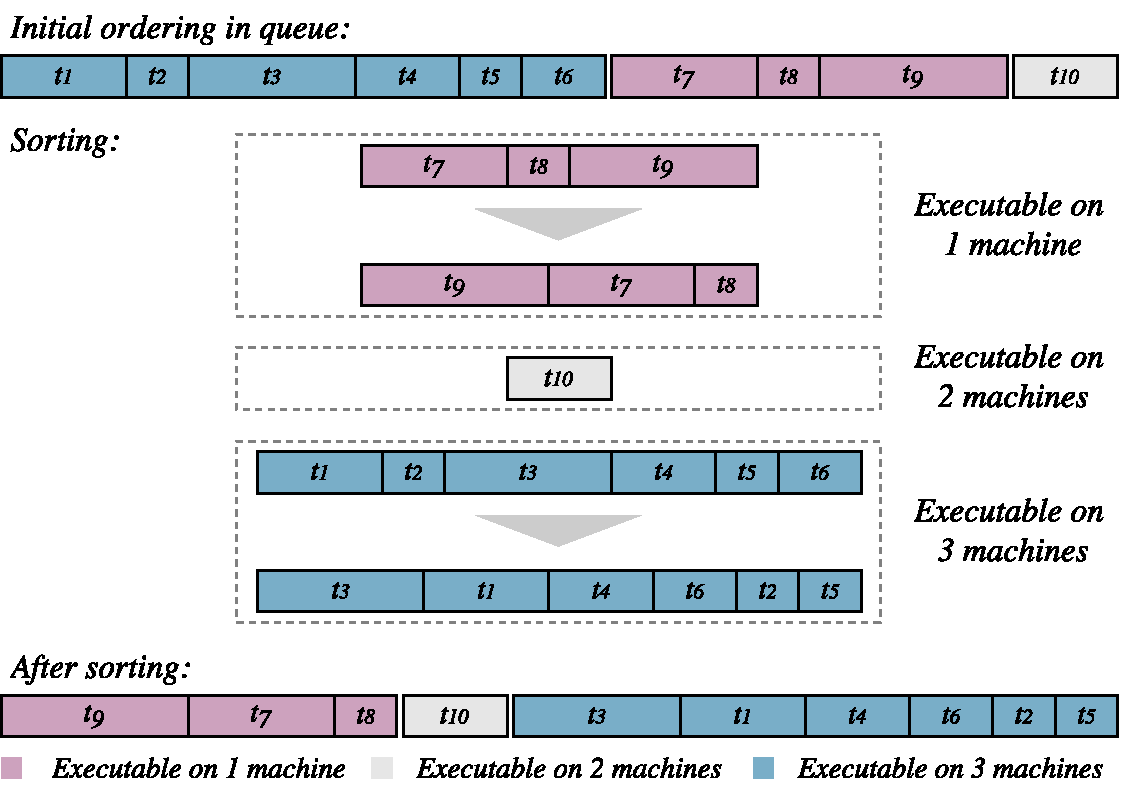
\includegraphics[width=\textwidth]{figures/new/sorting.pdf}
    \thisfloatpagestyle{plain}
    \caption{Sorting of Example Test Suite}
    \label{fig.sorted_test_suite}
\end{figure}

Figure \ref{fig.sorted_test_suite} illustrates how the sorting method works with the example test suite introduced earlier. Since $t_{7}$, $t_{8}$ and $t_{9}$ can only be executed on a single machine each, these are placed first in descending order of their duration. $t_{10}$, which can be executed on two machines comes after. Finally, tests $t_{1}$ through $t_{6}$, which can run on all of the machines, are ordered and added to the test list.






\vspace{7px}
\noindent \textbf{\betterfakesc{Initial Allocation}}\\
\noindent The initial allocation is a greedy algorithm, which means that it always makes a locally optimal choice in the hopes that it will give the best result in the end \cite{Algorithms}. Greedy algorithms are powerful and work well for an extensive spectrum of problems. Creating a greedy algorithm was a suitable choice for this problem.

This step creates the foundation of the test allocations. After being sorted, the test list is looped through, and the tests are allocated one by one, starting with the \emph{longest} of the tests that are executable on the \emph{fewest} machines. Each test is initially allocated to the machine that currently has the shortest overall duration among the machines that the test is executable on.

\begin{figure}[h]
    \centering
    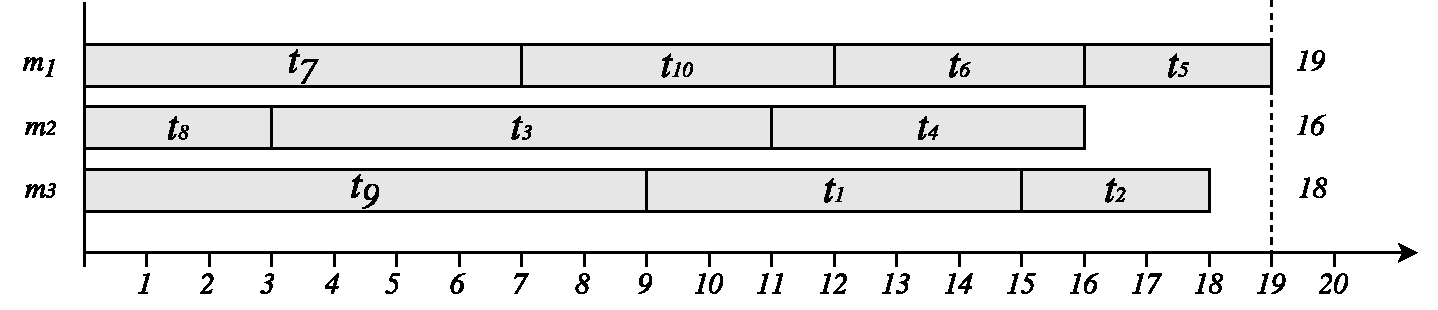
\includegraphics[width=\textwidth]{figures/new/initial_allocation2.pdf}
    %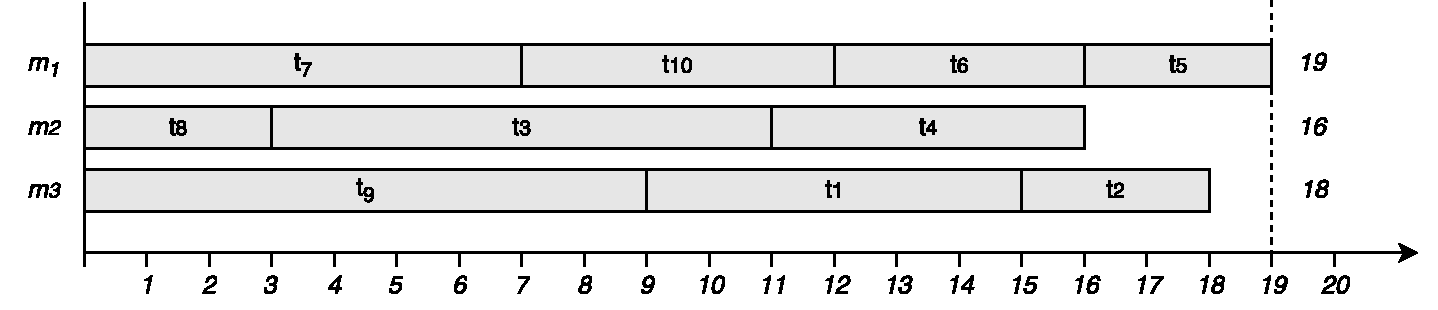
\includegraphics[width=\textwidth]{figures/initial_allocation.pdf}
    \caption{Initial Allocation of Example Test Suite}
    \label{fig.initial_allocation}
\end{figure}

Figure \ref{fig.initial_allocation} shows how the test suite is initially allocated among the test machines. $t_{9}$, $t_{7}$ and $t_{8}$ are first allocated to $m_{3}$, $m_{1}$ and $m_{2}$ one by one, as each of them can only be executed on that machine. $t_{10}$ can be executed on both $m_{3}$ and $m_{1}$, but as the latter currently has the shortest overall execution time, this is the machine it is allocated to. The remaining tests are allocated in the same way. After the initial allocation is finished, the overall execution time is 19. However, the total durations among the machines are slightly uneven, so there might be room for improvement. This will be examined in the last step of Opti-X.






\vspace{7px}
\noindent \textbf{\betterfakesc{Enhancement Iterations}}\\
\noindent Greedy algorithms are simple, yet efficient, and provide adequate results most of the time. However, they do not always yield optimal solutions. In order to improve the result, an additional step has been included in the Opti-X. This is the most complex element in the process.

The basic idea behind the iteration step is to find subsets of tests among two machines and swap the two subsets that will decrease the total duration of the two machines the most. The subject of each iteration is the machine that currently has the longest execution time. In the case of the example test suite, this is $m_{1}$. This will be referred to as the \emph{swapper}. Each of the remaining machines are addressed one by one, starting with $m_{2}$, which is a \emph{swappee} candidate. The tests that are currently allocated to the swapper, but also executable on the swappee candidate are retrieved, which in this case is $t_{5}$ and $t_{6}$. A list of all possible subsets from this set is then created. This is done by using Python's \emph{itertools} library. The same is done the other way around, with $t_{3}$ and $t_{4}$ for the swappee candidate. After this, we examine how each swap would affect the overall total duration of the two machines in question. After comparing all subsets, it is concluded that the best swap is $t_{5}$ and $t_{6}$ from $m_{1}$ for $t_{4}$ from $m_{2}$, which will decrease the overall duration among the two machines with 1 time unit. Since $m_{3}$ can not provide any better options, this swap is conducted. This process will repeat until there is no way to improve the allocations, which in this case is after one swap. In this example, \toolname \space found an optimal solution to the optimization problem. Figure \ref{fig.iteration} shows how the subset swap is conducted, and how it affects the overall duration.

Upon evaluating each swappee candidate, a naive best-case duration is calculated by adding the durations of all the tests from the two machines and dividing the sum by two. If the time used to search for the best swap exceeds the difference between the total duration of the swapper (here: 19), and this best scenario duration (here: $\frac{19+17}{2} = 18$), which in this case is $1$, we will continue to the next swappee candidate. This means that we will examine the subsets of $m_{2}$ for maximum 1 unit of time.

%In an attempt to save time, the subsets are sorted according to their total durations; the swapper subsets descending and the swappee subsets ascending. This ensures that the subsets with the longest total durations are attempted removed from the swapper first.

\begin{figure}[t]
    \centering
    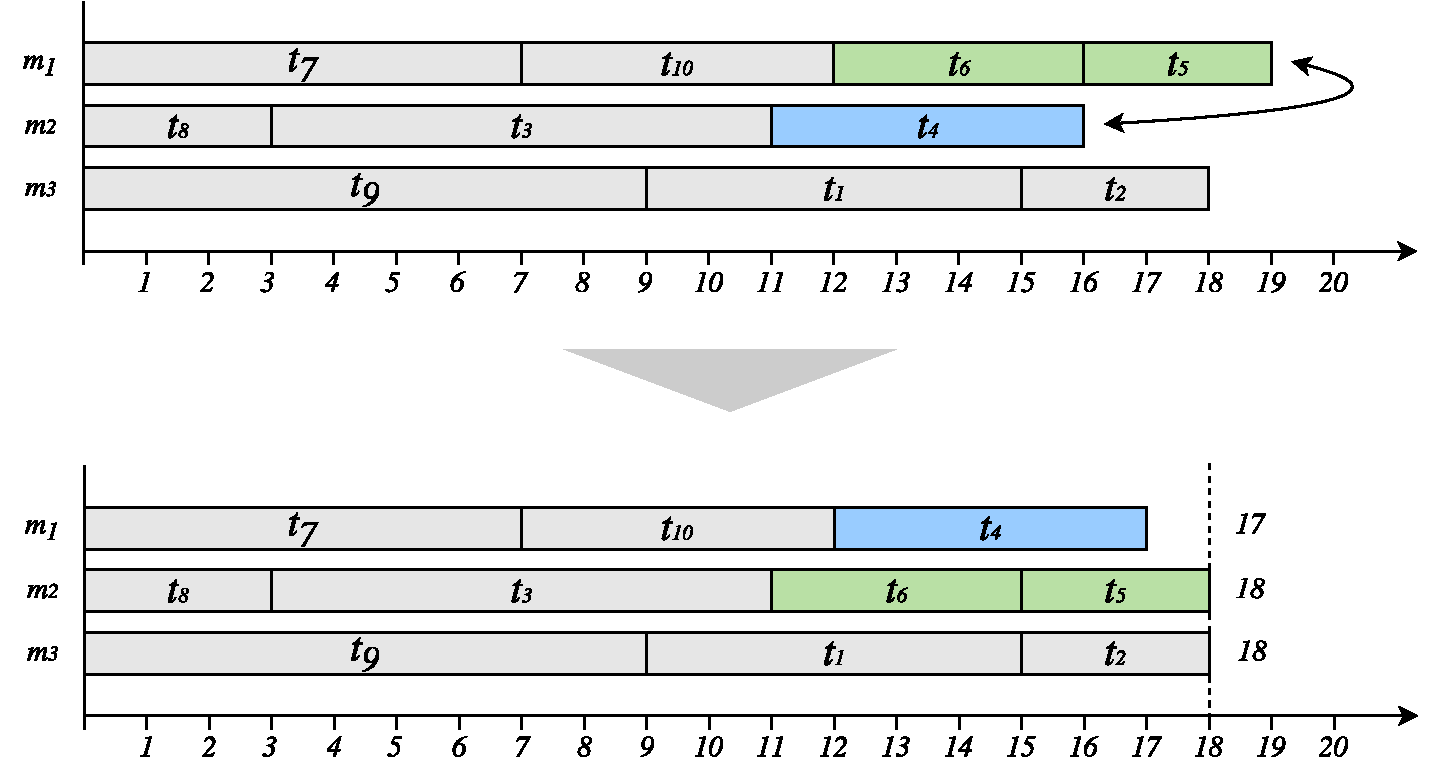
\includegraphics[width=\textwidth]{figures/new/iteration2.pdf}
    %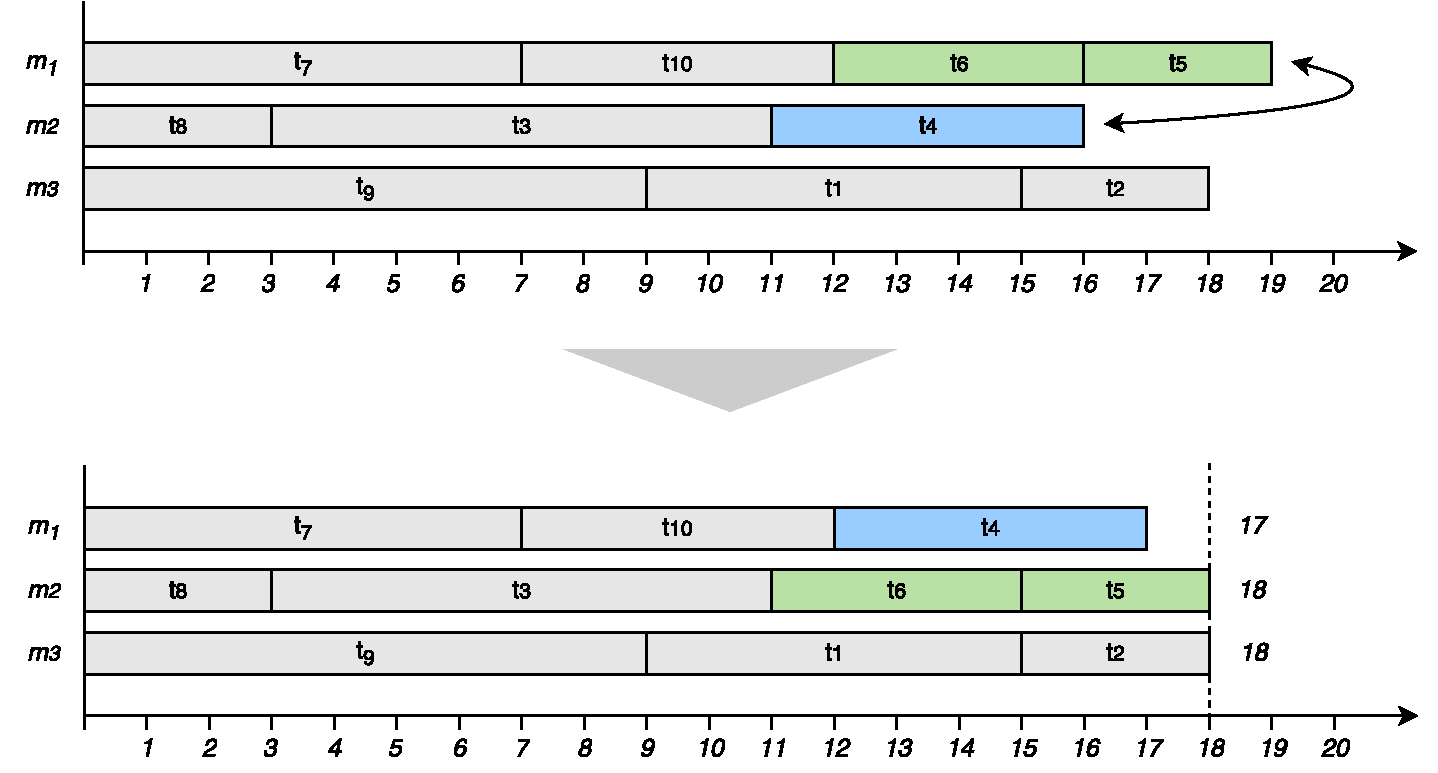
\includegraphics[width=\textwidth]{figures/iterations2.pdf}
    \caption{Enhancement Iteration of Example Test Suite}
    \label{fig.iteration}
\end{figure}

Sometimes, however, we want to stop the searching earlier, as continuing is no longer beneficial. For that reason, two stop criteria are introduced:

\begin{enumerate}
    \item When the iteration method is first called, a naive best-case overall duration value is calculated by dividing the sum of all test durations by the number of machines available. Once the time difference between this value and the maximum machine duration is exceeded, the iteration process will stop.
    \item There is a timeout set to 60 seconds. If the iterations still are not finished at this point, the method will be terminated, and the allocations arrived at that point will be kept.
\end{enumerate}

During the development phase, a clear problem stood out; creation of subset lists from extremely large interchangeable test sets between two machines could take several minutes, and sometimes even lead to memory leaks so that the whole system crashed. This was because there was simply too many possible subsets. To work around this problem, a restriction of the maximum size of the subsets had to be established. Through trial and error, the following was decided upon:

\[
\hfill
    f(x)=\left\{
        \begin{array}{l l}
          x         &   \hspace{20px} if \hspace{32px} x < 10\\
          20-x      &   \hspace{20px} if \ 10 \leq x < 20 \\
          1         &   \hspace{20px} if \ 20 \leq x
        \end{array}
    \right.
\hfill
\]

Thus, if the number of interchangeable tests are 19 or more, the subset list will only consist or singular tests in addition to the empty set. Although not optimal, this was a compromise that helped on the problem. This means that for large interchangeable sets, tests can only be swapped one against one or moved from one machine to another. It is therefore sensible to think that better swaps might exist, although identifying these would take too much time and potentially lead to memory leaks.  Figure \ref{fig.subsets} shows a plot of $f(x)$.

\begin{figure}[h]
    \centering
    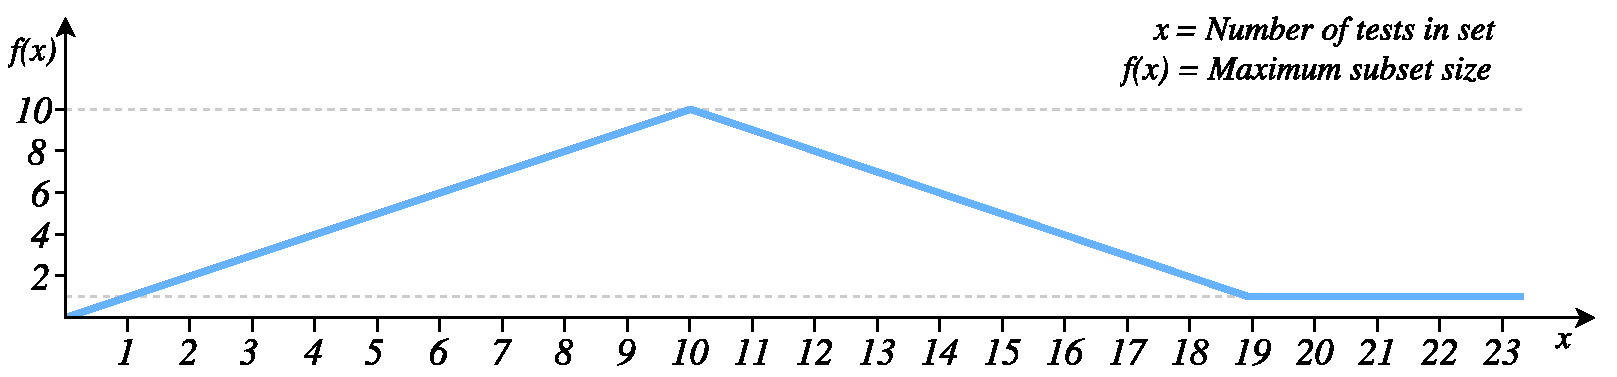
\includegraphics[width=\textwidth]{figures/new/subset_sizes.pdf}
    %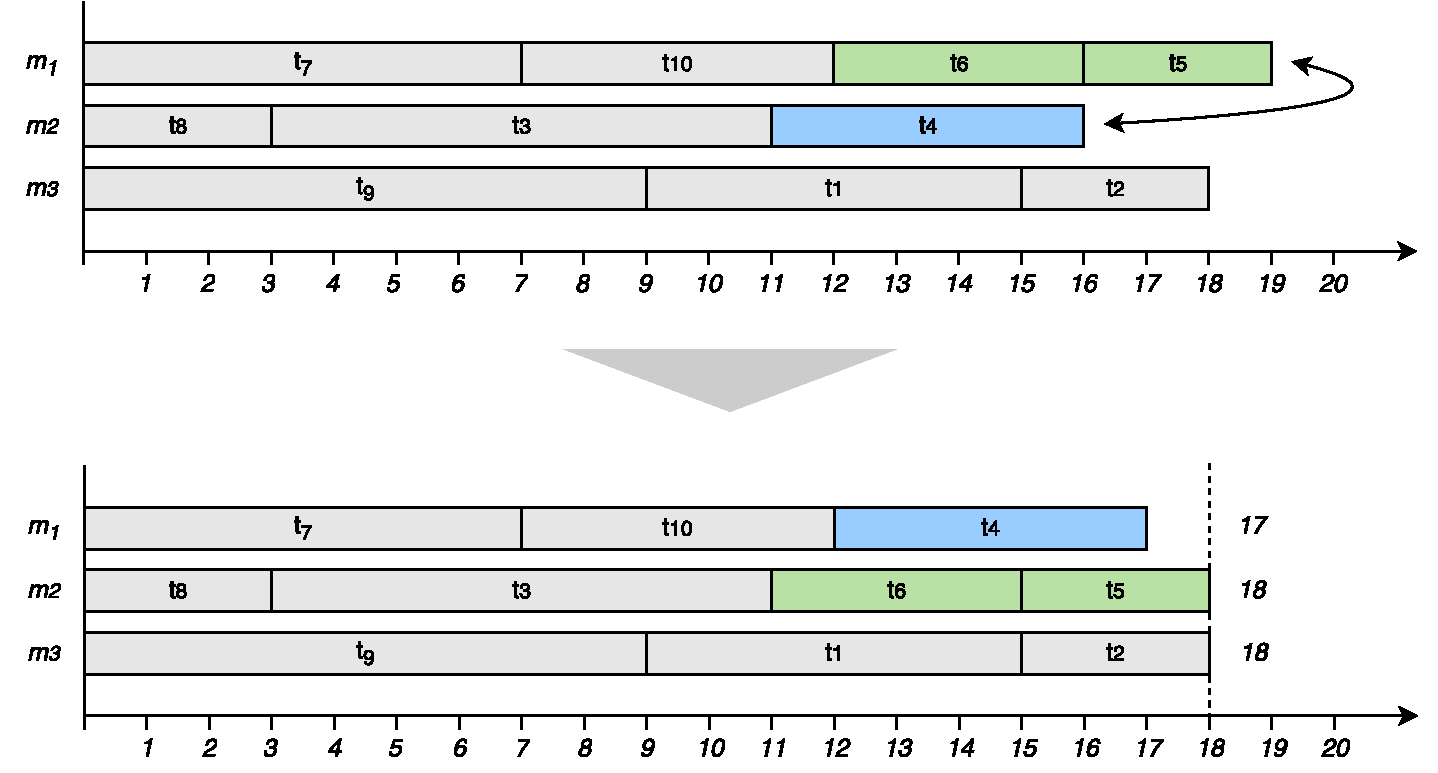
\includegraphics[width=\textwidth]{figures/iterations2.pdf}
    \caption{Maximum Subset Sizes}
    \label{fig.subsets}
\end{figure}

Because of the stop criteria described earlier and the subset size restriction, \toolname \space cannot \emph{guarantee} to find an optimal solution to the allocation problem. However, as explained in Section \ref{subsection.cp}, the objective of the optimization problem is to minimize the total time, which means that the time used to search for the best solution is also of high importance, and should be prioritized as such.

\subsubsection{OR-X}

The implementation of OR-X is of the same style as the OR-Tools example shown in \lstlistingname \space \ref{listing.or_tools} in Chapter \ref{chapter.technology}, but more complex. OR-X takes two lists; one containing the durations of the tests, and another containing which machines each test is executable on. OR-Tools does not support decimal values, so all values in the durations list must be converted to integer values. The \emph{executable on} list is nested, with one list belonging to each test. These inner lists contain binary values representing whether or not the test can be executed on a given machine. It is then added as a constraint that each test should be allocated to exactly one machine, and as the objective that the overall duration should be minimized.

However, there was one major issue upon the implementation of OR-X. It was not possible to interrupt or time out the \emph{NextSolution} method. For very small data sets, this was not a problem, but once the data sets grew slightly bigger and the combination possibilities grew rapidly, the method could take hours. This meant that a set of stop criteria had to be introduced. However, the problem could still not be solved by running the solver in a separate thread, as there is no integrated method of terminating regular threads in Python to the best of the authors knowledge. the problem was solved by introducing Python's \emph{multiprocessing} library.

The solving method is started as a \emph{Process} from the multiprocessing library. In order to allow two processes to share lists, a \emph{Manager} is needed, and to ensure synchronization, a \emph{Lock} has been used. \lstlistingname \space \ref{listing.orx_multiprocess} shows how these multiprocessing modules are used in OR-X.

\vspace{4mm}
\begin{lstlisting}[caption=OR-X Multiprocessing, label={listing.orx_multiprocess}]
from multiprocessing import Process, Manager, Lock

manager       = Manager()
allocations   = manager.dict()
max_durations = manager.list()
last_updated  = manager.list()
lock          = Lock()

// ...

p = Process(target=find_solution, args=(durations, executable_on, allocations, max_durations, last_updated, lock))
p.start()

while p.is_alive():
  if lock.acquire():
    if <stop criteria fulfilled>:
      p.terminate()
      break
    lock.release()

// ...

def solution_loop(self, durations, executable_on, shared_allocations, max_durations, last_updated, lock):
    // ...
    
    while solver.NextSolution():
      lock.acquire()
      // ...
      lock.release()
\end{lstlisting}

\noindent OR-X will be terminated if one of the following stop criteria are fulfilled:

\begin{itemize}
    \item The search for an enhancement has taken 100 times as long as it took to find the previous enhancement.
    \item The previous enhancement took 10 times as long to find than the enhancement itself.
    \item 60 seconds have passed (timeout).
\end{itemize}







%%%%%%%%%%%%%%%%%%%%%%%%%%%%%%%%
% SUBSECTION: Database
%%%%%%%%%%%%%%%%%%%%%%%%%%%%%%%%
\subsection{Database}

The relational database management system (RDBMS) SQLite can be regarded as a light-weight substitute to other SQL based database engines. Benefits to SQLite compared to these other database systems include its being self-contained and serverless, and the database is contained in a single disk file \cite{https://www.sqlite.org/about.html}. For convenience concerning submission, SQLite was the preferred choice for this project. However, another SQL database engine can replace it with little effort if needed.

As explained in Chapter \ref{chapter.technology}, Django data models define the database layout, and each model typically maps to an individual table in the database. SQL code for creating the database itself and the tables within it are all auto-generated by Django, based on the implementations of the models. If a m-to-n relation between two different models are defined in the model implementations, a separate relationship table is created in the database to cover this. The auto-generated SQL files covering creations and changes to the tables related to test automation are all placed under \emph{testautomation} $\rightarrow$ \emph{migrations} by default. When a change has been done to one of the models, a new migration can be created by performing a few shell commands \cite{https://docs.djangoproject.com/en/1.9/topics/migrations/}.

The database can be accessed either by writing raw SQL queries, or through Django's API for database abstraction. The former approach was first implemented in this system, but was then changed to the latter, as it was cleaner and more consistent with the implementation of the rest of the project. It was also interesting to use a different practice of database communications than the more commonly used raw SQL queries. \lstlistingname \space \ref{listing.db} shows a simplified example of how an \betterfakesc{insert} statement is conducted using this approach. In this example, the implementation of the \betterfakesc{Log} model is imported, and then an object of this type is created with pseudo values for a small set of attributes. Line 5 in the listing represents the transaction execution and commit. Note that implementation of such object creations includes several more attributes than what is shown in this example.

\vspace{4mm}
\begin{lstlisting}[caption=Database Communication Using Abstraction API, label={listing.db}]
from testautomation.models import Log
from datetime import datetime
 
l = Log(title='test1', result=1, execution_time=datetime.utcnow())
l.save()
\end{lstlisting}

\noindent In addition to providing excellent readability, the abstraction greatly decreases the required number of code lines needed to achieve the same result compared to executing raw SQL queries. This is because the database location does not need to be stated, connection with the database does not need to be programmatically established and then closed when the transaction is finished, and so forth. The abstraction takes care of all of this. The running time of the two approaches also proved to be approximately the same after testing both methods. Other types of queries such as \betterfakesc{Select}, \betterfakesc{Update} and \betterfakesc{Delete} are also supported with this API.

Information about test cases, test groups, schedules, logs as well as user information is all stored in various tables of the database. Figure \ref{fig.db_er} shows the Entity-Relationship (ER) diagram of the database.


\begin{figure}[p]
    \centering
    \thisfloatpagestyle{empty}
    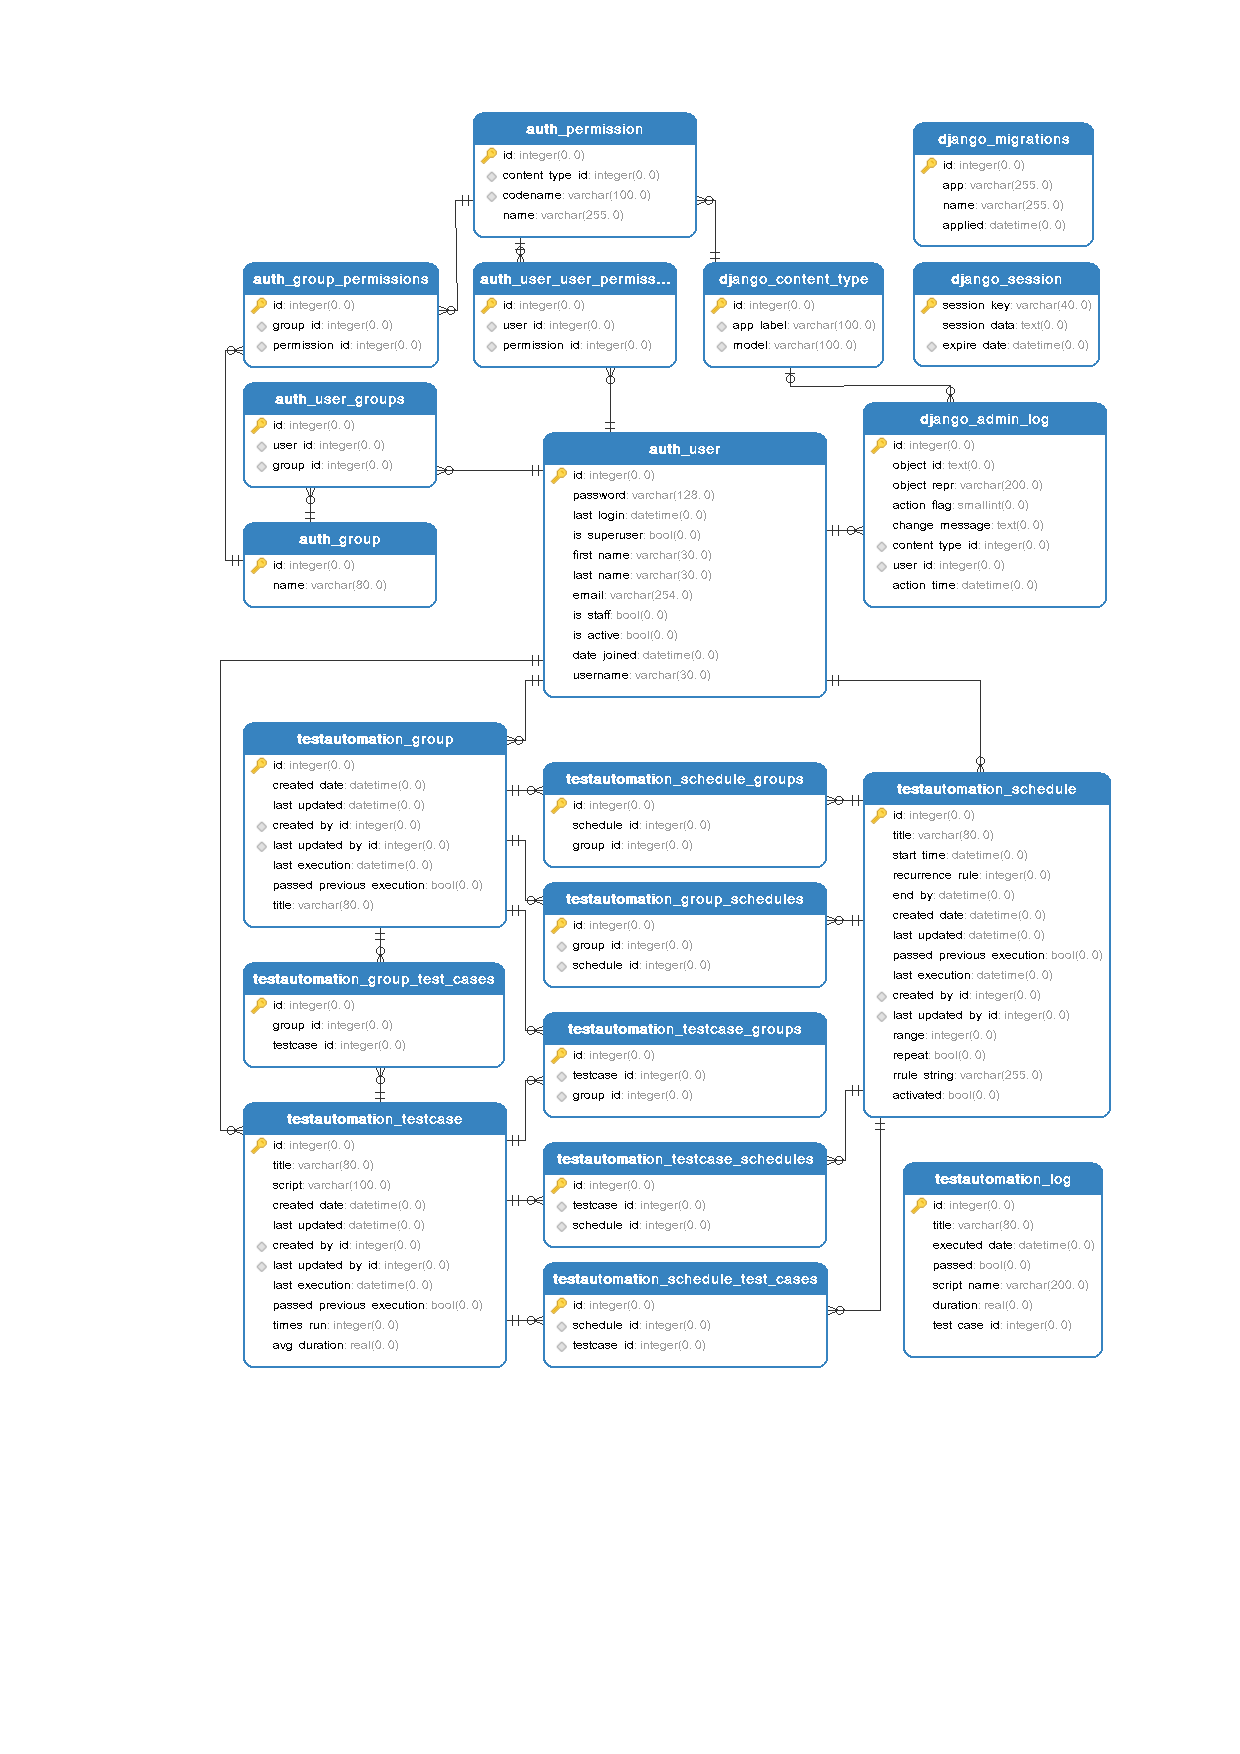
\includegraphics[width=\textwidth,height=\textheight]{figures/er_diagram.pdf}
    \caption{ER Diagram of Database}
    \label{fig.db_er}
\end{figure}

All timestamps stored in the database are in the Coordinated Universal Time (UTC) standard, which, as the name suggests, is universal, and therefore independent of time zones. The time zone used in the web service is set to 'Europe/Oslo' in the Django settings file. Whenever a timestamp is shown on screen, it is first converted to the specified time zone using Django's \emph{timezone} library. If the user is located in a different time zone than the one specified in the settings, a label explaining that the computer is \emph{xx} hours ahead or behind of server time is displayed next to any \emph{datetime} picker, such as in the schedule creation form.

\noindent Storing timestamps according to the UTC standard rather than the current time zone can be considered good practice for multiple reasons. Firstly, there can be no ambiguity. Confusion and misunderstandings related to conversion across different time zones will be avoided, which also means that timestamp calculations are simple. Further, there can be no invalid dates linked to daylight savings time. Moreover, if the server were to be moved to a different time zone, timestamps would have to be converted.





%%%%%%%%%%%%%%%%%%%%%%%%%%%%%%%%
% SUBSECTION: Dashboard
%%%%%%%%%%%%%%%%%%%%%%%%%%%%%%%%
\subsection{Dashboard}

\improvement[inline]{TODO: Write section intro}
\comment{\todo[inline]{TODO: Describe maybe a little bit more how django/django admin works? Some parts are automatic and some are implemented. Some stuff are overrided, some stuff are extended, etc}}

\subsubsection{Models}

With Django, data models provides the foundations on which database tables are created and maintained. A model implementation can be seen as a Python equivalent to an SQL \betterfakesc{Create Table} statement. Model implementations are translated to SQL and executed by Django. Each model, which is a subclass of \emph{django.db.models.Model}, represents a table in the database, and each model field represents a database field. Similar to SQL, the data type of each field along with any other specifications such as the maximum length of a text field, default values and help text can be passed as \emph{field option} parameters.

The models are located in \emph{testautomation} $\rightarrow$ \emph{models.py}. In this file, model specifications of test cases, groups, schedules and logs are implemented.

Additionally, models can contain elements that are not linked to the database, such as a field of which a value is based on a function that is performed each time the value is requested displayed. These functions can return primitive data types, but they can also contain HTML tags, so the content can be customized. Such functions are used in several of the models. For instance in the test case module, there are one function that query the \betterfakesc{Log} table in the database, and counts number of instances linked to the particular test case. Average duration and previous execution date are retrieved in a similar manner.

\vspace{4mm}
\begin{lstlisting}[caption=Model Implementation, label={listing.model}]
from django.db import models
 
class TestCase(models.Model):
    title = models.CharField(max_length=80)
    script = models.FileField(upload_to='scripts')
    
    def times_run(self):
        tr = # perform query
        return tr
\end{lstlisting}

\noindent \lstlistingname \space \ref{listing.model} shows a reduced adaption of how the test case model has been implemented. This model contains two model fields and a function. The \emph{script} field is of the type \emph{model.FileField}, and the directory that the files should be uploaded to is passed as a parameter. The file upload itself is taken care of by Django.





\subsubsection{Admin}

\improvement[inline]{TODO: Write introduction to this subsection}

\vspace{4mm}
\begin{lstlisting}[caption=Implementation of Model in Administrator Interface, label={listing.modeladmin}]
from django.contrib import admin
from .models import TestCase

class TestCaseAdmin(admin.ModelAdmin):
    list_display = ('title', 'times_run', 'avg_dur')
    search_fields = ['title',]
    fields = ('title', 'script')
 
admin.site.register(TestCase, TestCaseAdmin)
\end{lstlisting}

\noindent \lstlistingname \space \ref{listing.modeladmin} shows a very reduced interpretation of how the test case model is represented in the administrator interface. This adaption builds on the model implementation from \lstlistingname \space \ref{listing.model}. Model administrator representations are subclasses of \emph{django.contrib.admin.ModelAdmin}, and specifies how the model should be represented in the administrator interface. This interpretation specifies values of three of the many ModelAdmin options; which fields of the model should be displayed in the overview list of the test case module ('list\_display'), which fields should be searchable ('search\_fields') and which which fields should be present in the creation/change form ('fields'). Line 9 registers the model to the administrator interface with the specifications stated in the TestCaseAdmin class.

In the actual implementations of the model admin representations, a number of additional fields and specifications are also included. Custom forms with particular validation functionality can be integrated with the creation/change form. This has been done with test case objects to ensure that only test scripts that fulfill certain criteria can be uploaded. Admin actions are also implemented here.

\improvement{TODO: List and describe the implemented admin actions?}

\subsubsection{Issue Tracker Reporting}
\improvement[inline]{TODO}
\comment{TODO - JIRA Rest API, etc.}

\subsubsection{Management of Test Machines}
\improvement[inline]{TODO}

\subsubsection{Event Recurrence}
\betterfakesc{Rrule}, short for \emph{recurrence rule}, is a part of to a Python library called \emph{dateutil}, which provides an extension to Python's \betterfakesc{datetime} module. It  is a small and fast library used in \toolname \space to specify recurrence patterns of test executions. \betterfakesc{Rrule} instances can be implemented multiple ways. In this project, it is achieved through passing a string with a specific format, containing information about the desired recurrence constraints. This string is stored in the database, and can be used at any point to create an \betterfakesc{rrule} instance in order to inquire when the next event should take place. An example of such a string, how \betterfakesc{rrule} instances are created in this project, and how the next occurrence is retrieved, can be seen in \lstlistingname \space \ref{listing.rrule}.

\vspace{4mm}
\begin{lstlisting}[caption=Recursion Rule, label={listing.rrule}]
from dateutil.rrule import rrulestr
from datetime import datetime

rule_string = "DTSTART:20160615T160000\nRRULE:FREQ=WEEKLY"
rule = rrulestr(rule_string)
 
print rule.after(datetime.now())
 
>>> 2016-06-15 16:00:00
\end{lstlisting}

\noindent The string in the listing above is used to create an rrule instance in which the first occurrence is set to the 15\textsuperscript{th} of June 2016 at 4 pm, and repeats weekly. In addition to the recurrence properties shown in the listing above, the library provides an extensive number of recurrence options, including end date, occurrence count and interval.

\comment{
    \missingfigure[figwidth=\textwidth]{Screenshot of filled-in schedule form? With corresponding rrulestr?}
    
    The recurrence rule strings in this project are built dynamically when a schedule object is created or updated. If the schedule creation form shown in Figure \ref{fig.rrule} is submitted, it would produce the following 
}

The recurrence rule strings in this project are built dynamically when a schedule object is created or edited. In the test case, group and schedule modules of \toolname, recurrence rule strings are used to create \betterfakesc{rrule} instances, which again are used to find out the time of the next planned execution for the particular test case, group or schedule. \betterfakesc{Rrule} instances are also created by the controller to check when the next test run is scheduled.


\comment{
\subsection{Other?}
\change[inline]{
Include data flow - what happens from someone clicks "Execute now" and until the result is shown in the log? (FLOW CHARTS!)
How are Jira issues created?

Include a (detailed?) figure system architecture of how the system is integrated. Start by explaining how the different parts talk to each other. In the beginning, consider the controller as a unit, give more detailed descriptions of objects, listeners, algorithms, etc later.

How does the scheduling algorithm work? Try to be as academic as possible - use academic language when describing the algorithm; define the problem mathematically, use graphs and flow charts, use an example.

Two types of scheduling:
- Optimal allocation and scheduling of test cases in a test run
- Planned scheduling of future test run with recurrence option (rrule, rrulestr)
}

\comment{SELENIUM GRID is load balanced, but otherwise chooses which machine to execute a test on sporadically. There is no documented way of specifying which node to execute a specific test on, but it can be done by adding some unique information to each node upon setup, and to use the same piece of information in the capability section in the setup function of the test script. https://groups.google.com/forum/#!topic/selenium-users/PRsEBcbpNlM}

\todo[inline]{
Scheduling algorithm:

job-machine-matrix / test case-node matrix (binary) (shows which machine can run each test case, which machines each test case can run on)}

    [
        \hfill
        \mathbb{M} = \kbordermatrix{
                  & tc_{1} & tc_{2} & tc_{3} &        & tc_{n} \\
            m_{1} & x_{11} & x_{12} & x_{13} & \dots  & x_{1n} \\
            m_{2} & x_{21} & x_{22} & x_{23} & \dots  & x_{2n} \\
                  & \vdots & \vdots & \vdots & \ddots & \vdots \\
            m_{d} & x_{d1} & x_{d2} & x_{d3} & \dots  & x_{dn}
        }
        \hfill
    ]



http://stackoverflow.com/questions/5674253/a-task-job-scheduling-problem

\comment{
\info[inline]{
Constraints:
- Each test case must be executed once and once only
- Machines can execute test cases in paralell
- Execution time is assumed to be machine independent
- Each machine can only execute one test case at a time
- Heterogeneous environment (at least not necessarily homogeneous) - different OS and OS versions, different browsers and browser versions - not all test cases can be executed on each machine

Objective: Minimizing running time


From TC-Sched:
time-constrained cumulative scheduling constraint-based technique because 1) it allows
us to keep fine-grained control on the time allocated to the
constraint solving process (i.e., time-constrained), 2) it encodes
exclusive resource use with constraints (i.e., constraint-based),
and 3) it solves the problem by using the CUMULATIVES constraint.
The TC-Sched method is composed of three elements,
namely, the constraint model described in Section III-A, the
search procedure described in Section III-B, and the timeconstrained
minimization process described in Section III-C.


Constraints:
-Non-cumulative scheduling: Two test cases cannot be executed at the same time on a single machine.
-Non-preemptive scheduling: The execution of a test case cannot be temporarily interrupted for the running machine to execute another test case instead.
-Non-shared resources: When a test case uses a global resource, no other test case using the same resource can be executed at the same time.
-Machine-independent execution time: The execution time of a test case is assumed to be independent of the machine on which it is run. This is a reasonable assumption for test cases in which the time is dominated by external physical factors such as a robot’s motion, the opening of a valve, or sending an Ethernet frame. Such test cases typically have execution times that are uncorrelated with machine performance (e.g., CPU type, CPU frequency, operating system). In any case, a sufficient over-approximation of the execution time will satisfy the assumption.


EXPERIMENTAL EVALUATION

This section presents our findings from experimentally evaluating TC-Sched. To this end, we address the three following
research questions:

RQ1: How does the solution provided by TC-Sched compare with simpler scheduling methods in terms of the time needed to execute the schedule? RQ1 states the crucial question of wether using strong constraint optimisation tools is useful or
not in a context where cheaper-to-run methods are available at almost no cost of implementation.
RQ2: For TC-Sched, will an increased investment in the solving time reduce the overall time of a CI cycle? This question
is about finding the most appropriate trade-off between the solving time and the execution time of the test schedule.
RQ3: Can TC-Sched effectively handle industrial cases which contain up to hundreds of test cases and tens of machines?}
}
}